\chapter*{\FontH{\Huge Pinarella}}
\addcontentsline{toc}{chapter}{Pinarella}
\lettrine[lines=3]{\color{red}P}{}inarella war ein Schmetterling. Träge lag sie wie jeden Morgen auf dem Regal im Wohnzimmer der Familie Emil und liess sich die Sonne auf die Flügel scheinen. Sie gähnte so laut das Schmetterlingsdamen eben können und blickte sich gelangweilt im Zimmer um. Pinarella war nämlich kein einfacher Schmetterling, nein, sie bestand aus einem Körper aus Holz und die Flügel waren aus bunter Folie gemacht. Schön sah das zwar aus, aber zum Fliegen taugte so ein Körper nicht. Cornelia, die Tochter der Emils hatte Pinarella gebastelt, als sie so ungefähr in der dritten Klasse gewesen war. Aber das ist jetzt schon viele Jahre her, Cornelia hatte selbst schon zwei Kinder und mit denen war sie gerade zu Besuch bei ihren Eltern. Eigentlich wohnte Pinarella gar nicht auf dem Regal, sondern hing für gewöhnlich an einer Schnur über dem Ofen. Aber das letzte Mal als Cornelia mit den Enkelinnen dagewesen war, ist sie beim Spielen auf dem Boden gelandet und von da hat sie jeman auf das Regal gelegt. Bisher hatte sich noch niemand die Mühe gemacht, sie wieder aufzuhängen, aber das war Pinarella egal. Beide Orte sind genau gleich langweilig, so viel war klar. Deswegen war es auch ganz gleichgültig, wo sie gelagert wurde.


Spielen konnte sie allerdings auch bei den Emils. Besonders Jette, die jüngste Tochter von Cornelia machte das sehr gerne.  Jette war allerdings noch zu jung, um die Schönheit Pinarellas zu verstehen. Sonst würden sie wahrscheinlich nicht gar so garstig und nachlässig mit ihr umgehen. Mal wurde sie an den Flügeln gezogen, die dann umständlich von Frau Emil wieder festgeleimt werden mussten, dann wurde sie unachtsam unter einem Berg Legosteine vergraben. Und einmal wurde sie sogar mit auf die Pergola genommen und dann dort vergessen. Die ganze Nacht fror Pinarella ganz fürchtlerlich.

Jette war allerdings ein liebes Kind, das wusste Pinarella, deswegen nahm sie ihr das alles auch nicht übel. Sie war einfach noch zu jung. So viel wusste Pinarella über die Menschen: wenn sie klein sind, überlegen sie manchmal nicht, was so alles passieren kann, wenn sie dies und jenes machen. Gerade gestern ist Jette in alleine in ihr Stühlchen geklettert und dabei sehr unsanft abgestürzt. Das war ein Weinen! Und Jette hatte sich selbst bestimmt nicht mit Absicht weh getan, hatte Pinarella überlegt und so ging es wohl auch mit ihr, wenn Jette ihr mal wieder einen Fühler abgebissen hatte.

Auf dem Regal war Pinarella jetzt zwar sicher vor Jette, aber eben auch alleine. Jette war viel zu klein, um sie so weit hoch zu kommen. Lieber wieder einen Flügel verlieren, dachte Pinarella, als den ganzen Tag hier zu liegen. 

\begin{figure}[ht]
\centering
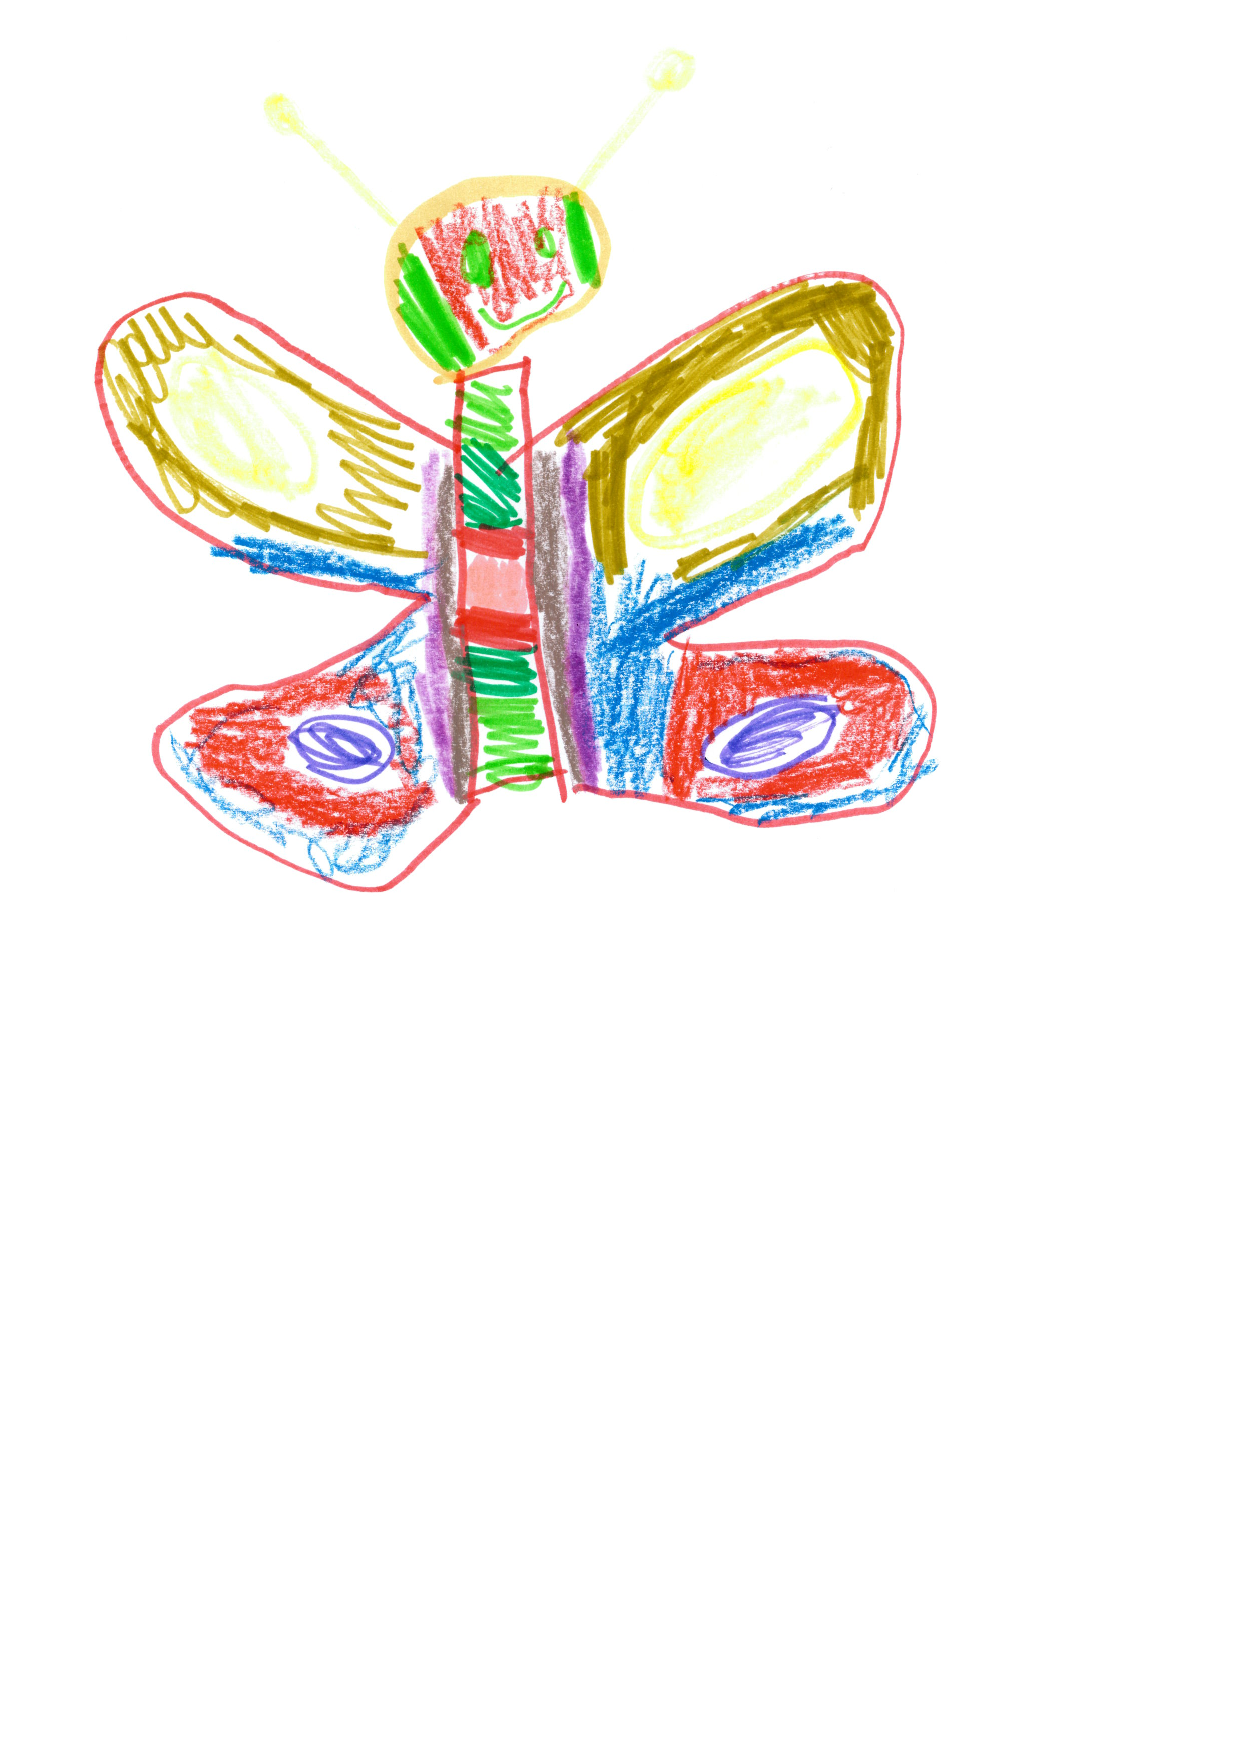
\includegraphics[width=.8\textwidth]{bilder/pinarella.pdf}
\end{figure}

\enquote{Schade} seufzte Pinarella, \enquote{wirklich schade, dass ich kein richtiger Schmetterling bin. Es ist ja schon lustig, mit Jette zu spielen, aber die ist einfach so selten zu Besuch. In der Zwischenzeit ist es doch immer sehr langweilig. Da wäre es ja doch viel lustiger, wenn ich hinaus fliegen könnte in die Welt, um mit anderen Schmetterlingen zu spielen.} 

An diesem Morgen war Jette mal wieder sehr früh munter geworden. Cornelia, die Jette selbstverständlich nur \enquote{Mama}  nannte und sie waren im Wohnzimmer und Cornelia war wieder eingeschlafen. Pinarella hatte das gar nicht gemerkt. Jette sass auf dem Boden und versuchte vergeblich ihrem Püppchen die Hosen anzuziehen. Wenn man erst zwei Jahre alt ist, klappt so etwas manchmal noch nicht so gut und ausserdem waren es sowieso Hosen für eine viel kleinere Puppe. Die Sache klemmte und damit auch die Lust von Jette, weiter mit der Puppe zu spielen. Gerade als sie sich umsah, um zu sehen, womit man als nächstes so spielen könnte, hörte sie die Klage von Pinarella. 

\enquote{Was ist denn mit dir los?} fragte Jette. Pinarella war verwirrt. Schon oft hatte sie versucht mit Menschen zu reden, aber so laut sie auch geschrieen hatte, nie hat sie jemand gehört.

\enquote{Kannst Du mich verstehen?} fragte sie daher ganz ungläubig. 

Jette nickte bloss. 

\enquote{Mir ist langweilig.} sagte Pinarella, niemand spielt mit mir, meine Flügel sind schon voller Staub.

\enquote{Dann komm doch hier zu mir geflogen!} schlug Jette vor, die den Unterschied zwischen einem echten Schmetterling und einem gebastelten noch nicht so genau kannte. Und obwohl Jette das gar nicht so genau interessierte, erklärte Pinarella ihr den Unterschied. Ihr war das nämlich wichtig. Jette verstand nicht alles, aber eines war klar: Pinarella wollte auch gerne fliegen können, um mit anderen Schmetterlingen spielen zu können. Das verstand Jette sogar gut, sie spielte ja auch am liebsten mit anderen Kindern.

\enquote{Dann helfe ich Dir!} beschloss Jette, hatte aber noch keine Ahnung, wie. Aber das ist normal bei Zweijährigen. Die beschliessen immer Sachen, von denen sie noch nicht wissen, wie man das dann genau macht. Zuerst musst Pinarella mal von dem Regal herunter, das war offensichtlich. Das Regal war schon sehr hoch, sogar noch höher als Papa gross ist, schätzte Jette. Der konnte einen aber hoch nehmen, wenn man die Arme in die Luft streckt, Regale machen so etwas wohl aber nicht. Jette hatte bereits ein bisschen Lebenserfahrung. Und die sagte ihr auch, dass man wohl etwas zu Hilfe nehmen musste.

Die beide sahen sich im Zimmer um, was wohl genau diese Hilfe sein könne. Jette hatte plötzlich eine Idee. Wenn sie mit dem Wasserhahn vom Waschbecken spielen wollte, schob sie sich immer das Schemelchen hin und stieg darauf. Für das Waschbecken war sie nämlich auch noch zu klein.  Aber das Schemlechen war natürlich im Badezimmer und wenn man dort hin wollte, würde Mama bestimmt munter werden. Pinarella und Jette mussten seufzen. Beinahe gleichzeitig sahen sich die beiden an, dann zum Stuhl, dann wieder sich. So leise wie eine Zweijährige eben kann, lief Jette zu dem Stuhl und schob ihn so vorsichtig wie möglich in Richtung Regal.

\enquote{Mach keinen Quatsch!} Mama war von dem Quitschen munter geworden, drehte sich aber zum Glück nochmals auf die Seite und schlief weiter. Jette und Pinarella hatten den Atem angehalten, den Jette mit einem lauten {\it Pffff.} jetzt wieder raus liess. Das war knapp. Wenn Mama gemerkt hätte, was Jette vor hat, wäre sie bestimmt dagegen gewesen. Ganz leise kletterte Jette jetzt auf den Stuhl. Noch immer reichte sie nicht bis oben hin. Zum Glück sah Jette sofort dendem Rückenkratzer vom Opa, den konnte sie nehmen und tatsächlich! Es klappte! Jette kam gerade so bis an das obere Ende des Regals, konnte Pinarella an einem Fühler erwischen und zog sie vom Regal herunter.

Mit einem leisen {\it Plopp} landete Pinarella auf der Couch, aber zum Glück weit genug von Mama entfernt. Jette kletterte vom Stuhl herunter, was gar nicht so einfach war, nahm Pinarella, öffnete das Fenster und mit einem lauten 

\enquote{Jippie, flieg Pinarella!} war Jette den Holzschmetterling aus dem Fenster.

Natürlich konnte Pinarella nicht fliegen. Sie stürzte jäh ab und raste in Richtung Boden. 

\enquote{Da wird bestimmt noch mehr kaputt gehen, als nur ein Fühler.} dachte Pinarella. Gerade in dem Moment ging die Sonne hinter den Bergen auf. Und genau als Pinarella in der Luft war, traf sie der allererste Sonnenstrahl des Tages. Pinarella konnte ihn auf ihren Flügeln spüren und instinktiv zuckte sie zusammen und da geschah es. Ihre Flügel bewegten sich! Erst langsam, dann immer schneller und noch bevor Pinarella auf dem Boden aufschlagen konnte, flog sie. Aus der Spielzeugpinarella war ein richtiger Schmetterling geworden. Höher und immer höher flog sie, fast so hoch wie das Haus und wieder runter zu dem Blumen auf der Wiese und einfach immer weiter. Jette jubelte vor Freude und Mama, die von ihrem geschrei munter geworden war, guckte ganz verschlafen, was da los ist.

\enquote{Und nur wegen einem Schmetterling machst du so einen Lärm, dass du mich wecken musst?} Jette musste lächeln, Mama hatte nicht gemerkt, dass sie selbst den Schmetterling gebastelt hatte, der da geflogen war. \hfill {\color{red}\decofourleft}
